\section{The Actor Model}
As described in \cref{}\jenote{find afsnit om hvorfor vi skal køre parallelt} most simulations are very heavy and need HPC to operate at resonable speeds. Furthermore HPC runs parallel to utilize the performance of multiple processors. On modern architectures parallelism is achieved via system threads. Threads is one of multiple ways to optain concurrency, but they are obligatory when trying to achieve parallelism, at least in current modern usage \jenote{indsæt kilde}. As described in \cref{sec:models}, models are used as the conceptional still images of simulations and general dynamic behaviour. We therefore need a way to create models that can operate parallel. Threads are not easy to use to abstract over the definition of models. Since this language focuses heavily on models and simulations a more compatible abstraction is needed.

If we look at the definition given earlier about models, they consist of a general theory and a description of objects and systems. This is a definition is very similar to how object oriented programming works, where all programs consists of objects, with fields and methods, and systems are build around these. It is not surprising that this is a property of object oriented programming, since it has been designed to model the real world.
Because of this it would be very beneficial to use a concurrent abstraction that has the same base where everything is objects.
The actor model is often described as the object oriented concurrency model. The rest of this section will describe why this is the case, but because of its similarity to object oriented thinking the actor model was found to be the best concurrency model for simulations and therefore also The Language Described in this Report.

The actor model is a concurrency model, which first appeared in 1973 in the report \enquote{A Universal Modular ACTOR Formalism for Artificial Intelligence} by Carl Hewitt, Peter Bishop and Richard Steiger \cite{Hewitt:1973}. This section will explain the model generally, be compared to alternative concurrency models and a few implementations of the model will be briefly described.

\subsection{Model}
The actor model is focused on the fact that any computational behaviour, be it functions, processes or data structures, can be modelled as a single behaviour; sending messages to actors.
An actor in this context is a process, which has its own isolated state, used to store values and modify its own behaviour, and a message box, for receiving messages. An actor can only share information by sending messages, asynchronously, to other actors.
Actors are very similar to the communicating sequential processes (CSP) described in C.A.R. Hoare's publication \enquote{Communicating Sequential Processes} \cite{hoare1985communicating}. Actors, though, have a few well-defined behaviours in response to receiving a message, where CSPs are free to exhibit other behaviour. An actor can, in response to a message: 

\begin{enumerate}
  \item Send a finite number of messages to other actors.
  \item Spawn a finite number of new actors.
  \item Change its own behaviour for the next message that is received.
\end{enumerate}

In figure \ref{fig:actor}, a model of an actor based program can be seen.

\begin{figure}[htbp]
  \centering
  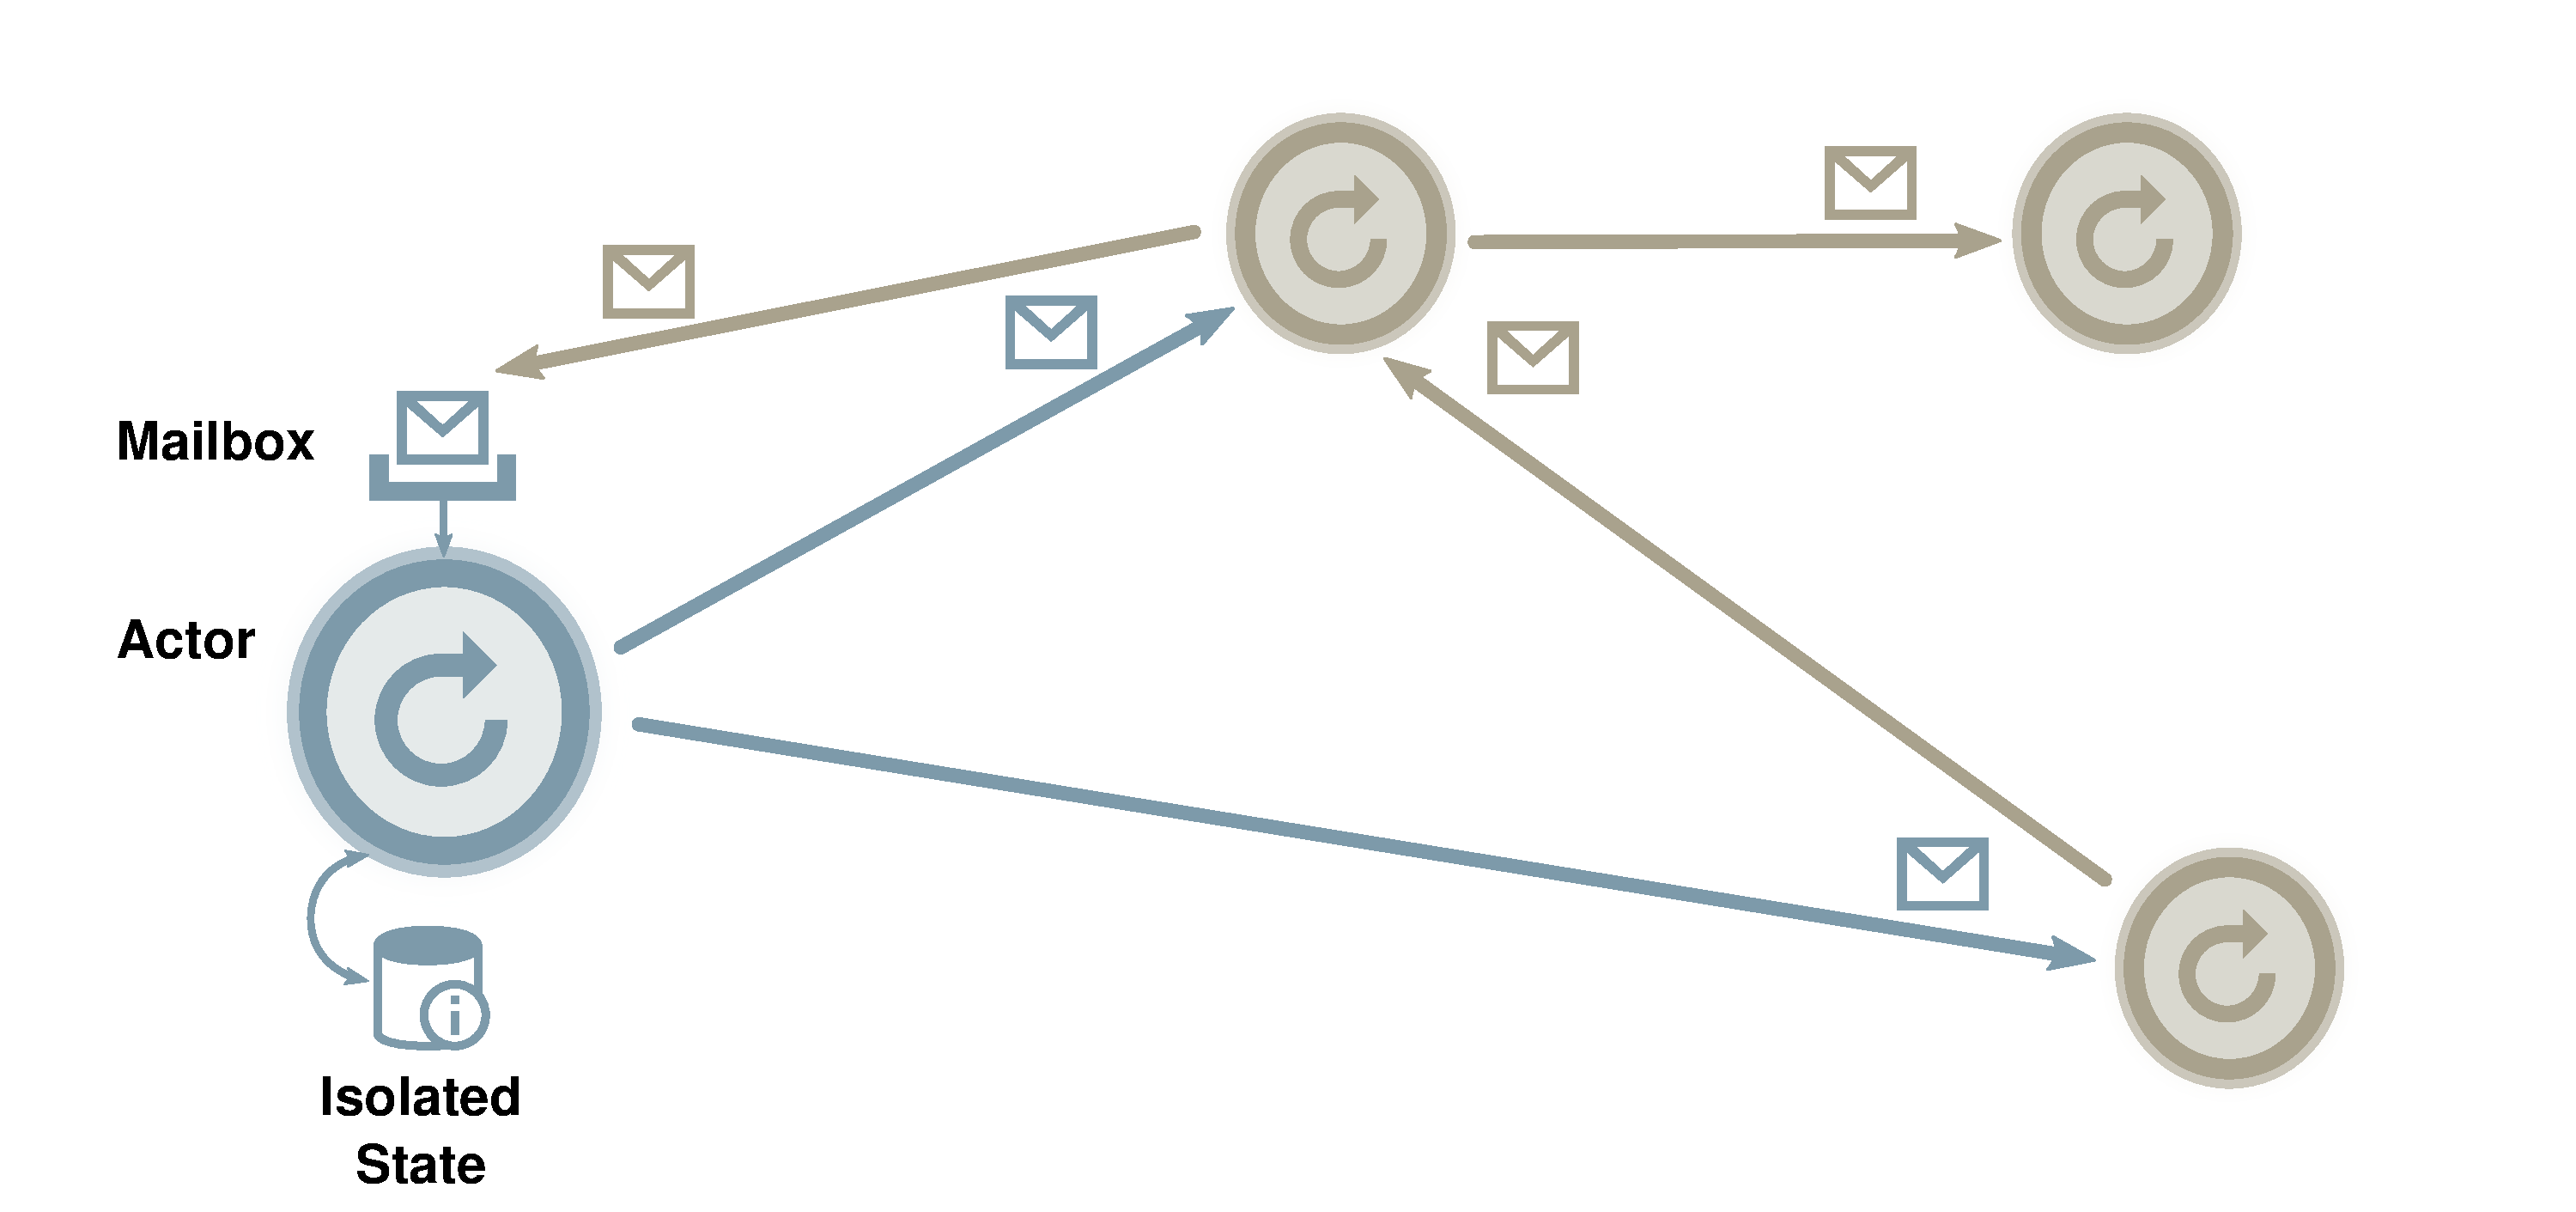
\includegraphics[width=\textwidth]{Images/actors.pdf}
  \caption{A model of an example program using actors. The nodes in this graph represent actors and the edges represent messages being sent.}
  \label{fig:actor}
\end{figure}

\subsubsection{Theoretical Basis} 
As mentioned, actors are very similar to, and have their theoretical roots in CSP.
In CSP, a program is composed of processes that operate independently from each other. These processes share information by messages passing. In Hoare's original version of CSP, each process was defined as a sequential series of instructions, however later versions of CSP typically allow a process' logic to consist of other processes.

While many aspects of CSP and the actor model are identical, there are some differences. In CSP, all processes are anonymous, while in the actor model, actors have identity. Sending a message to an actor can be regarded as largely equivalent to invoking a method on an object in the object-oriented world view. Since CSP does not have named processes, communication is done via named channels, as seen in programming languages such as Go and OCaml. 
In CSP, communication is synchronous, i.e. the receiver of a message must be ready to receive the message, before it can be sent by the sender. In the Actor model, all communication is asynchronous, meaning a message can be sent, without considering whether the receiving end is ready or not.

\subsubsection{Adding Logic}
One of the main features of the actor model is, as Hoare describes it, the ability to add knowledge to a system, without rewriting the existing knowledge. This means that if a developer is interested in adding a logical step in the business logic of his system, this can be achieved by merely adding an actor, which can perform the logical operations, that are to be added, and then adding that actor as a link in the flow of logic.

\paragraph{Example}
We have a system which can read a CSV-file and print it to stdout. This can be implemented by letting \emph{Reader} and \emph{Printer} be actors.

\begin{table}[htbp]
\centering
\begin{tabular}{ | c | c | c | }
\hline
Step & Reader & Printer \\\hline
1 & \textbf{Read CSV-file} & \textit{Wait for message} \\\hline
2 & \textbf{Send data to Printer} & \textit{Wait for message}\\\hline
3 & \textit{Wait for message} & \textbf{Receive data from Reader}\\\hline
4 & \textit{Wait for message} & \textbf{Print data to stdout}\\\hline
\end{tabular}
\label{ReadPrintExample}
\caption{A simple example showing two actors reading a file and printing the contents, respectively.}
\end{table}

At some point we decide that we wish to format our data before printing it. To do so, we create and incorporate a new actor, \emph{Formatter}, which changes the flow of execution in this manner:\\

\begin{table}[htbp]
\centering
\begin{tabular}{ | c | c | c | c | }
\hline
Step & Reader & Formatter & Printer \\\hline
1 & \textbf{Read CSV-file} & \textit{Wait for message} & \textit{Wait for message} \\\hline
2 & \textbf{Send data to Formatter} & \textit{Wait for message} & \textit{Wait for message}\\\hline
3 & \textit{Wait for message} & \textbf{Receive data} & \textit{Wait for message} \\\hline
4 & \textit{Wait for message} & \textbf{Format data} & \textit{Wait for message} \\\hline
5 & \textit{Wait for message} & \textbf{Send data to Printer} & \textit{Wait for message} \\\hline
6 & \textit{Wait for message} & \textit{Wait for message} & \textbf{Receive data}\\\hline
7 & \textit{Wait for message} & \textit{Wait for message} & \textbf{Print data to stdout} \\\hline
\end{tabular}
\caption{An example of extending the logic of \cref{ReadPrintExample} by also formatting the contents of the file, using another actor.}
\end{table}

Notice that in adding the new logic, the only existing logic that was changed is the actor whom \emph{Reader} sends data to.

\subsubsection{Concurrency}
The actor model is, as previously stated, inherently concurrent.

\paragraph{Isolated State}
As actors only communicate via message passing, each actor can have its own isolated state. This means that no two actors share any data, meaning problems such as race conditions, starvation and deadlocks are avoided entirely. These problems would lead to programmers having to deal with the administration of serialising access to the data, by means of locks, mutexes, semaphores or similar concurrency control mechanisms.

\paragraph{Separated Logic}
In the actor model, each actor has its own subprogram, which is only known by the actor itself and can be run in an infinite loop. A consequence of this is that an arbitrary actor never depends on another actor, meaning an actor's logic is isolated from the rest of the system and can be regarded as an atomic concurrent part of the system.

\paragraph{Example}
To demonstrate the actor model's ability to deal with classical concurrency problems, an example will be shown here. This example, shows the problem of phantom reads, which can be a big problem in data-rich, highly parallel systems. In the example, a collection is being accessed by two concurrent processes, or threads. One tries to read the collection, and the other tries to delete it.

We start off, with the problem shown in a typically imperative way, using threads. See \cref{table:eximpThreads}.
%
\begin{table}[htbp]
\centering
\begin{tabular}{ | c | c | c | }
\hline
Step & Thread A & Thread B \\\hline
1 & \textbf{Read first element in collection} & \textit{No operation} \\\hline
2 & \textbf{Process element} & \textbf{Delete collection}\\\hline
3 & \textbf{\color{red} Read second element in collection} & \textit{No operation}\\\hline
\end{tabular}
\caption{An example of a phantom read using two threads.}\label{table:eximpThreads}
\end{table}

As seen in this example, thread B is able to delete the collection, while thread A is still using it. This means that once thread A tries to access the second element of the collection, it runs into the phantom read problem and would likely terminate and throw an exception.

To demonstrate the same functionality that these threads are performing, using actors, we need three actors, \emph{Holder}, \emph{Reader} and \emph{Deleter}. \emph{Holder} contains the collection, \emph{Reader} reads and processes the elements in the collection and \emph{Deleter} wants to delete the collection.
%
\begin{table}[htbp]
\centering
\begin{tabular}{ | m{0.7cm} | m{3.5cm} | m{4cm} | m{3cm} | }
\hline
Step & Holder & Reader & Deleter \\\hline
1 & \textit{Wait for message} & \textbf{Send request to \emph{Holder}} & \textit{Wait for message} \\\hline
2 & \textbf{Send collection to \emph{Reader}} & \textit{Wait for message} & \textbf{Send \enquote{delete} to \emph{Holder}} \\\hline
3 & \textbf{Delete collection} & \textbf{Read first element in collection} & \textit{Wait for message} \\\hline
4 & \textit{Wait for message} & \textbf{Read second element in collection} & \textit{Wait for message} \\\hline
\multicolumn{4}{ | c | }{...}\\\hline
n & \textit{Wait for message} & \textbf{Read n\textsuperscript{th} element in collection} & \textit{Wait for message} \\\hline
\end{tabular}
\caption{An example of avoiding a phantom read by using actors.}\label{table:exActorPhantom}
\end{table}

As can be seen in \cref{table:exActorPhantom}, using actors to model this system ensures that there are no phantom reads. This is ensured, by the fact that actors never share data; therefore, an arbitrary actor can never corrupt, or delete, the data of another.

\subsubsection{Supervisors}
Most implementations of the actor model implement a form of a supervisor-worker relationship. This means that every actor has a supervisor, typically their parent, to whom they report failures. The supervisor then has to deal with the failure, by for example restarting the failed actor.
Supervisors in the actor model works very well with the \enquote{fail fast}-principle of programming, meaning, in the actor model, that an actor will not try to continue operation or correct an error when encountering a failure. An actor that has failed will, as soon as the failure is detected, report the failure to its supervisor and halt operation, moving the responsibility of handling the failure up the supervision tree.

\subsection{Implementations}\label{sub:implementations}
The Language Described in this Report is not the first language to implement the actor model. Two popular implementations, a mature one and a more current one, will be described here, to provide insight in the typical syntax and semantics of actors.

\subsubsection{Erlang}
When talking about the actor model, one cannot escape the subject of Erlang. Erlang was one of first languages to fully incorporate the actor model as the main model of concurrency. Erlang is a purely functional language, developed for the telecommunications industry, where a lot of concurrent processes have to be handled. 

Actors in Erlang, or processes as they are called, are controlled by a few very simple constructs; actors can be spawned using the built-in spawn-function, the spawn-function takes three arguments, the module in which the actor is contained, the function that defines the behaviour for the actor and an initial message. You can send messages to actors using the bang-operator (!) and you can define an actor's behaviour in a receive-block.

In Erlang, an actor's parent is it's supervisor, if one chooses to use the supervisor module available. Using the supervisor module in Erlang gives the programmer the ability to choose different strategies to be used when a child actor fails. These strategies are:
\begin{enumerate}
  \item Respawn the failed child
  \item Respawn all children when one fails
  \item Respawn all children after the child in the start order of the children
\end{enumerate}

\paragraph{Example}
To demonstrate the use of actors in Erlang, a simple example is shown in listing \ref{lst:ErlExample}. This program has only one actor, which counts the number of \enquote{incr}-messages it has sent.

\begin{lstlisting}[style=erlang, caption={A simple message-counter in Erlang.}, label=lst:ErlExample]
-module(countMsgs).
-export([run/0, counter/1]).

run() ->
  S = spawn(countMsgs, counter, [0]), %spawn S as counter-actor
  sendMsgs(S, 10000), %send 10000 messages to S
  S.
  
counter(Sum) -> %function-definition for counter-actor
  receive
    value -> io:fwrite("Value is ~w~n", [Sum]);
    incr -> counter(Sum+1)
  end.

sendMsgs(_, 0) -> true; %base case
sendMsgs(S, N) -> %recursive function to send N messages to actor S
  S ! incr, %send incr to S
  sendMsgs(S, N-1).
\end{lstlisting}

\subsubsection{Akka}
A more modern approach to the actor model is taken in Akka, a concurrency toolkit for Scala and Java.
In Akka, an actor is just an object, which extends Akka's Actor-class and implements a receive method. One difference in the receive-method from Erlang's receive-block is that Akka's receive-method is exhaustive, meaning that the programmer has to define behaviour for all possible messages that an actor can receive. 

Creating an actor in Akka is done by calling the \emph{actorOf}-method, on an actor or an instance of \emph{ActorSystem}, which acts as the parent of top-level actors. The \emph{actorOf}-method takes a \emph{Probs} as an argument, \emph{Probs} is just an object containing properties for an actor, such as the definition of the actor. Just like Erlang, messages are sent using the bang-operator.

In Akka, supervisors have the ability to handle failures in child actors in the following manner:
\begin{enumerate}
  \item Ignore failure and resume operation
  \item Restart the child from initial state
  \item Terminate the child, without respawning it
  \item Fail (move failure up supervision tree)
\end{enumerate}

\paragraph{Example}
To demonstrate Akka's implementation of actors, the same example shown in listing \ref{lst:ErlExample} will be implemented in Scala, using Akka, in listing \ref{lst:AkkExample}.

\begin{lstlisting}[style = scala, caption={A simple message-counter in Scala.}, label=lst:AkkExample]

import akka.actor.Actor
import akka.actor.Probs

class Counter extends Actor{ //definition of counter-actor
  var count = 0
  def receive = {
    case "incr" => count += 1 //if actor receives "incr", increment count
    case "value" => println(s"Value is $count")
    case other => println(s"Error: Cannot understand message $other") //default case
  }
}

object Main extends App {
  val mySystem = ActorSystem("MySystem")
  val myCounter = mySystem.actorOf(Probs[Counter], name="MyCounter") //create counter-actor as top-level actor
  def main(args:Array[String]){
    for (i <- 1 to 10000) { //send 10000 messages to myCounter
      myCounter ! "incr"
    }
  }
}
\end{lstlisting}

\subsection{Summary}
The actor model is a model for concurrency formalised by Carl Hewitt, based on the work of C.A.R. Hoare. The actor model provides an abstraction over concurrent processes, where locks, mutexes, semaphores and the like are unnecessary. The actor model's abstraction also solves some of the classical problems with concurrency, such as phantom reads. The actor model integrates very well with functional languages, as seen in \cref{sub:implementations}.
